% This is LLNCS.DEM the demonstration file of
% the LaTeX macro package from Springer-Verlag
% for Lecture Notes in Computer Science,
% version 2.2 for LaTeX2e
%
%\documentclass[12pt]{llncs}
%\documentclass[envcountsame,oribibl,11pt]{llncs}
\RequirePackage{amsmath}
\documentclass[runningheads,a4paper]{llncs}
%\documentclass[runningheads,a4paper]{llncs}
%\usepackage[hmargin=1in,vmargin=1.25in]{geometry} 

\usepackage{amsmath, amssymb}
\usepackage{algorithm,algorithmic}
\usepackage{makeidx}  % allows for indexgeneration
\usepackage{graphicx,epsfig,color}
\usepackage{boxedminipage}
\usepackage{multicol} 
\usepackage{enumerate}
\usepackage{diagbox}
\usepackage{float}
\usepackage[table]{xcolor}
\usepackage{multirow}
\usepackage{longtable}
%\usepackage{titlesec}

\setcounter{secnumdepth}{5}
% To use "Arial" font, use the following 2 lines
%\renewcommand{\rmdefault}{phv} % Arial
%\renewcommand{\sfdefault}{phv} % Arial

% The following statement specifies the amount of space between
% paragraphs. Other reasonable specifications are \bigskipamount and \medskipamount.
%\setlength{\parskip}{\smallskipamount}

% The following statement controls the line spacing.  
%\renewcommand{\baselinestretch}{1.0}

% TRACK CHANGE
% ------- Bar -------
%\begin{changebar}
% The proposed scheme
%\end{changebar}
% ------- Highlight -------
%\hl{scheme} 
% ------- Strikeout -------
%\st{framework}
%\usepackage{soul}
%\sethlcolor{green}
%\setstcolor{red}
%\usepackage[color]{changebar}
%\cbcolor{blue}

\begin{document}

%\bibliographystyle{abbrv}	% [1] A. Author. Article name, ...
\bibliographystyle{acm}	% [1] AUTHOR, A. Article name. ...
%\bibliographystyle{alpha}	% [Las98] Firstname Lastname. Article title. ... [alphabetical order]
%\bibliographystyle{apalike} 	% [Author, 1990]
%\bibliographystyle{amsplain}	% [1] Firstname Lastname, Italicized Article Name, ... 
								%        [authors in alpha order, underscore for repeated author]
%\bibliographystyle{ieeetr}	% [1] F. Writer. "Article name", ... [in order of reference]
%\bibliographystyle{plain}	% [1] Firstname Lastname. ...
%\bibliographystyle{siam}	% [1] A. AUTHOR, Italicized Article Name, ...
%\bibliographystyle{unsrt}	% [1] Firstname Lastname. Article name. ... [in order of reference]

%
\frontmatter          % for the preliminaries
%
\pagestyle{headings}  % switches on printing of running heads
\addtocmark{Title of The Paper} % additional mark in the TOC
%
\mainmatter              % start of the contributions
%
\title{A Survey on Trust in Autonomous Systems \\ 
}
%
\titlerunning{A survey on Trust}  % abbreviated title (for running head)
%                                     also used for the TOC unless
%                                     \toctitle is used
%
\author{\large Shervin Shahrdar and Mehrdad Nojoumian   %\inst{1} \thanks{Research supported by X.} 
%and Name-2 %\inst{2} \thanks{Research supported by X.}
}

\authorrunning{ Shervin Shahrdar  \& Mehrdad Nojoumian
}   % abbreviated author list (for running head)

\institute{
Department of Computer \& Electrical Engineering and Computer Science \\ Florida Atlantic University, Boca Raton, FL, USA \\
\email{sshahrda@fau.edu}, \url{www.shervinshahrdar.com} \\
\email{mnojoumian@fau.edu}, \url{http://faculty.eng.fau.edu/nojoumian/}
}

\maketitle
\begin{abstract}

\noindent As a result of the exponential growth in technology and computing in the past couple of decades, autonomous systems are becoming more relevant in our daily lives. As these autonomous systems evolve and become more complex, the concept of trust in such systems becomes a major challenge that affects the performance, and reliability of such systems. Many prior studies have indicated that currently, humans have a very low trust-level in the fully autonomous robots. Similarly, trust between autonomous systems plays a major role in their performance. In this meta-analysis, we will explore various research and trust models in order to show why trust management is a very challenging aspect of future AI technologies.

\vspace{10pt}
\textbf{Keywords:} Trust Function, Reputation Systems, Autonomous Systems, Multi-Agent Systems
\end{abstract}

%\addtolength{\parskip}{1.6ex}
%\parindent 0pt

%-------
\section{Introduction} 
\label{ShervinTrustSurvey_introduction}
The rapid growth in technology has resulted in the automation of many day to day tasks that humans had to perform themselves just decades ago. From ATMs (Automated Telling machines) to industrial robots used in factories, automation continues to aid humans with repetitive, difficult, and monotonous tasks. This technological advancement introduces newer and more complex robotic concepts, and automated systems in different areas of our lives including our homes, daily commute, workspace, military, and many other areas every day.

As these automated systems evolve, their levels of complexity increase overtime, and their involvement in various aspects of human life introduces the concept of human-robot trust. Studies have indicated that one of the most important challenges for successful integration of advanced autonomous systems and AI technology in human civilization, will be the management and the development of this mutual trust \cite{beer2014toward}.

In this paper, we will provide a step by step, comprehensive analysis and explore various concepts and related studies, as well as experimental techniques proposed by researchers in this field, in order to understand how the human-robot trust management works, and how we can improve it. Additionally, we will explore the trust between autonomous systems (Agents) in section 3.

\section{Definitions}
\subsection{What is an Autonomous System?}
First, an autonomous system needs to be defined. This definition keeps changing everyday as the related technology grows exponentially \cite{schaefer2013perception}.

Merriam Webster dictionary defines `autonomy' as  ``The quality or state of being self-governing; especially: the right of self-government''. The concept of Autonomy has existed for thousands of years, in many different areas including philosophy, sociology, politics, and technology. In fact, the second part of the term Autonomous, \textsl{nomos}, means `law' in  Greek. An autonomous entity ``creates its own laws''. \cite{MerriamWebsterAtn}. 

We need to narrow down this definition, as this it is very broad and applies to many different areas and concepts. Perhaps the term that we are looking for is `autonomous robots'. Autonomous robots are defined as, ``intelligent machines capable of performing tasks in the world by themselves, without explicit human control.'' \cite{Bekey:2005:ARB:1088950}

\begin{figure}
	\centering
		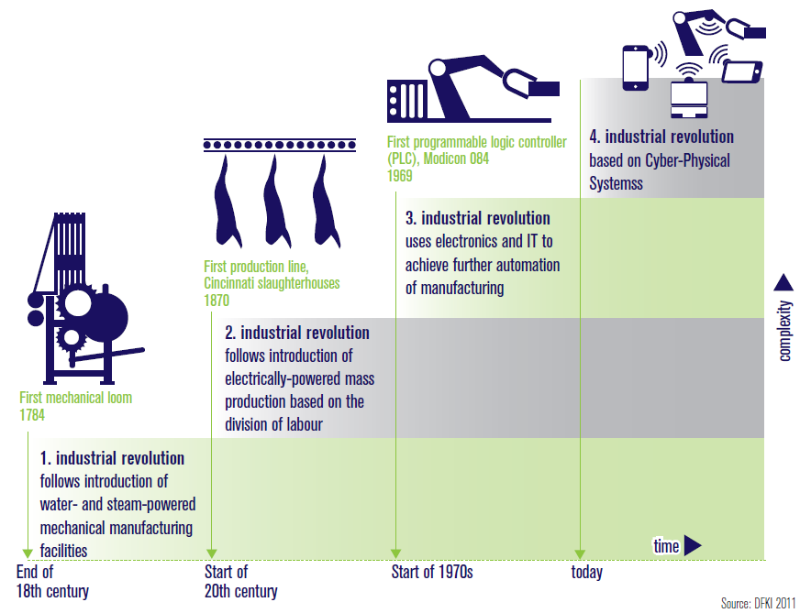
\includegraphics[width=\textwidth]{Figures/EvolutionOfAutomation.png}
	\caption{Evolution of Automation \cite{CyberSecurityInIndustry}}
	\label{Trust_Function}
\end{figure}
Although automation was introduced to human civilization many years ago, and widely used after industrial revolution in early 1800s \cite{IndustrialRevolution}, Autonomous systems, and Industrial Robots are relatively new terms that were introduced merely decades ago, and their definitions are evolving everyday, as technology advances. In this paper, our main focus will be on Autonomous Robots and Autonomous Agents which are a highly advanced form of automated machines that have a high degree of self-awareness, and are capable of independently performing tasks which were previously done by humans.

\subsection{What is Trust?}
`trust' is a concept that has many different definitions in various contexts such as psychology, sociology, and Economics. Currently, there is no uniform definition of `trust' in the context of psychology, or other areas \cite{adams2003trust}. Prior research indicates that there are over 300 definitions in various research areas, and in the context of Human-Robot relationships, which is our focus in this paper, there are more than 30 definitions. These definitions include `human interpersonal trust', `automation trust', `trust in software agents'', and many others \cite{schaefer2013perception}. 

Although there are complex definitions of trust documented based on the area of the research,  we shall focus on the simplest, domain-agnostic definition. A very simple, generic definition of `trust' would be: ``A firm belief in the reliability, truth, or ability of someone or something'' \cite{oxfordDicTrust}. If we consider this simple definition, then, in our research context, the definition of trust would be: ``A strong human belief in the reliability, truth, or ability of an autonomous system''. The `Autonomous system' in this case could be any kind of a self aware machine that has a high degree of autonomy. Some concrete examples would be human trust in self driving cars (SDC), autonomous planes, battlefield robots, rescue robots, autonomous software agents, and so on.

\section{Review of Literature: Trust in Autonomous Systems}
In this section, we will review, and categorize previous studies that are in the domain of human-robot trust relationship.

\subsection{Trust Between Humans and Autonomous Systems}

\subsubsection{Human-Robots}
As previously stated, many studies have shown that currently, the level of trust between humans and autonomous systems is very low. That means in serious situations, humans tend to not let fully autonomous systems take control. A study that explores the low level of human-robot trust, is done by Daniel Stormont (2008) \cite{stormont2008analyzing}. In this study, the factors that affect the trust between humans and robotic systems are analyzed. The study concluded that it is not just `trust' that determines the usability, but `confidence' also plays a significant role. One of the reasons the level of confidence in autonomous systems is very low is due to their low level of reliability. As cited in this paper, ``A 2004 study of commercially available ruggedized robots operating in
field conditions showed a mean-time-between-failures
(MTBF) of 12.26 hours and an availability rate of 37\%''\cite{carlson2004investigation}. This means, that if the robotic systems reduce their failure rate, their reliability will increase, thus, the human confidence and trust in them will increase. Of course this study was done in 2004. It is clear that due to recent advancements in robotic systems, the MTBF should be definitely less than 37\%. For example, when the first fatal car accident was reported for Tesla self driving cars, it became a topic of discussion in the media. Although these accidents are rare, companies like Tesla and Google learn the nature of the accident, and work on reducing the failure rate in the future models. \cite{TeslaFatalAccident}

In his research, Mr.Stormont (2008) also believes that another factor affecting the trust between humans and fully autonomous systems would be their unpredictability. It is known that in various hazardous circumstances such as battlefields and rescue missions, the unpredictability of robots becomes a critical problem for human supervisors. It has been argued that the autonomous nature of robots, and their decisions making could be a positive trait, since they could react faster to certain dangers compared to humans, but the problem arises when life and death of humans will depend on the choices of a robot; Questions such as ``should life and death decisions be made
by an autonomous system?'' will emerge. In the 2008 study, a simulation of robots assisting firefighters in a hazardous fire situation was discussed. It was concluded that even though firefighters did not initially trust these helper robots, as the mission went on, and they got tired, their reliance and trust in the robots increased, as they helped them extinguish the fire. 
\begin{figure}
	\centering
		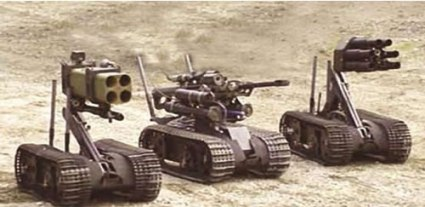
\includegraphics[scale=0.6]{Figures/3robots.jpg}
	\caption{Example of autonomous and semi-autonomous robots used in military \cite{autonomousArmedRobots}}
	\label{MilitaryRobots}
\end{figure}

Another study conducted by Mr. Babak Esfandiari and his colleague, Mr. Sanjay Chandrasekharan \cite{esfandiari2001agents} thoroughly examined and proposed ``simple
mechanisms for trust acquisition based on a very basic and general definition of trust.'' According this this study, the majority of views on the definition of trust are divided into two groups: Cognitive views, and mathematical views. Mr. Esfandiari argues that both of these views have something in common: both of them see `trust' as a variable, that also has a threshold for an action. This action is called cooperation. The mathematical definition of `trust' provided by this study is: ``Trust is a function T between any two agents of a set A of agents''. These agents can be humans, or robots, or autonomous systems, and so one. This study also provides a concept called `Trust Acquisition'. Given an example of previously defined mathematical function: T(Alice, Bob) (Trust between Alice and Bob), Trust Acquisition is described as ``the process or mechanism that allows the calculation and update of T. In our
definition, acquisition is not necessarily an 'increase' of T.''. This study provides various methods of Trust Acquisition:
\begin{enumerate}
	\item Trust Acquisition by Observation
	
	Mr. Esfandiari argues that Trust Acquisition can be obtained by performing `Bayesian Learning'. This means that agents observe, and consider that past actions of other agents, and decide whether to perform an action or not. This paper provides an example of two agents, RoboCop robots John and Mary. John has the ball, and is deciding whether or not pass the ball to Mary, or just shoot the ball himself. If John is able to review the past performances of Mary, and compares them with his own performance, and performs a statistical analysis, he will be able to make a decision.
	\item Trust Acquisition by Interaction
	
	In Trust Acquisition by Interactions protocol, agent 1 asks a bunch of pre-determined questions from agent 2. Agent 1 already knows the answer, thus, the trust will be acquired based on the the number of correct answers provided by agent 2.
	\item Trust Acquisition Using Institutions
	This study provides an example of humans trusting police officers wearing uniforms. If a person sees another person equipped with a gun who is wearing a uniform, he will automatically trust that person, because the trust is already established by the institution. However, if he sees a person not wearing a uniform and carrying a gun, he needs to make more calculations to trust this person.
	
\end{enumerate}


In a 2011 paper, Peter A. Hancock et al. provided a comprehensive analysis of factors affecting trust in ``Human-Robot Interaction (HRI)'' \cite{hancock2011meta}. This study categorizes factors that affect the trust in HRI into three different categories: human related, Robot related, and environmental variables, and each category has sub categories. Human related factors include training, expertise, situational awareness, demographics etc. Similarly, robot-related factors are behavior, dependability, reliability, level of automation, failure rates, false alarms, and transparency, and attribute based factors such as location, personality, adaptability, robot type, and Anthropomorphism (having human traits). Environmental factors include team work, culture, communication, shared mental models, task type, task complexity, multi-tasking, physical environment. This paper discovered that robot performance has the biggest impact on trust in the context of HRI, and tweaking the robot performance has a direct impact on trust. For example, if an autonomous robot improves its performance, the value of trust will increase.

\begin{figure}
	\centering
		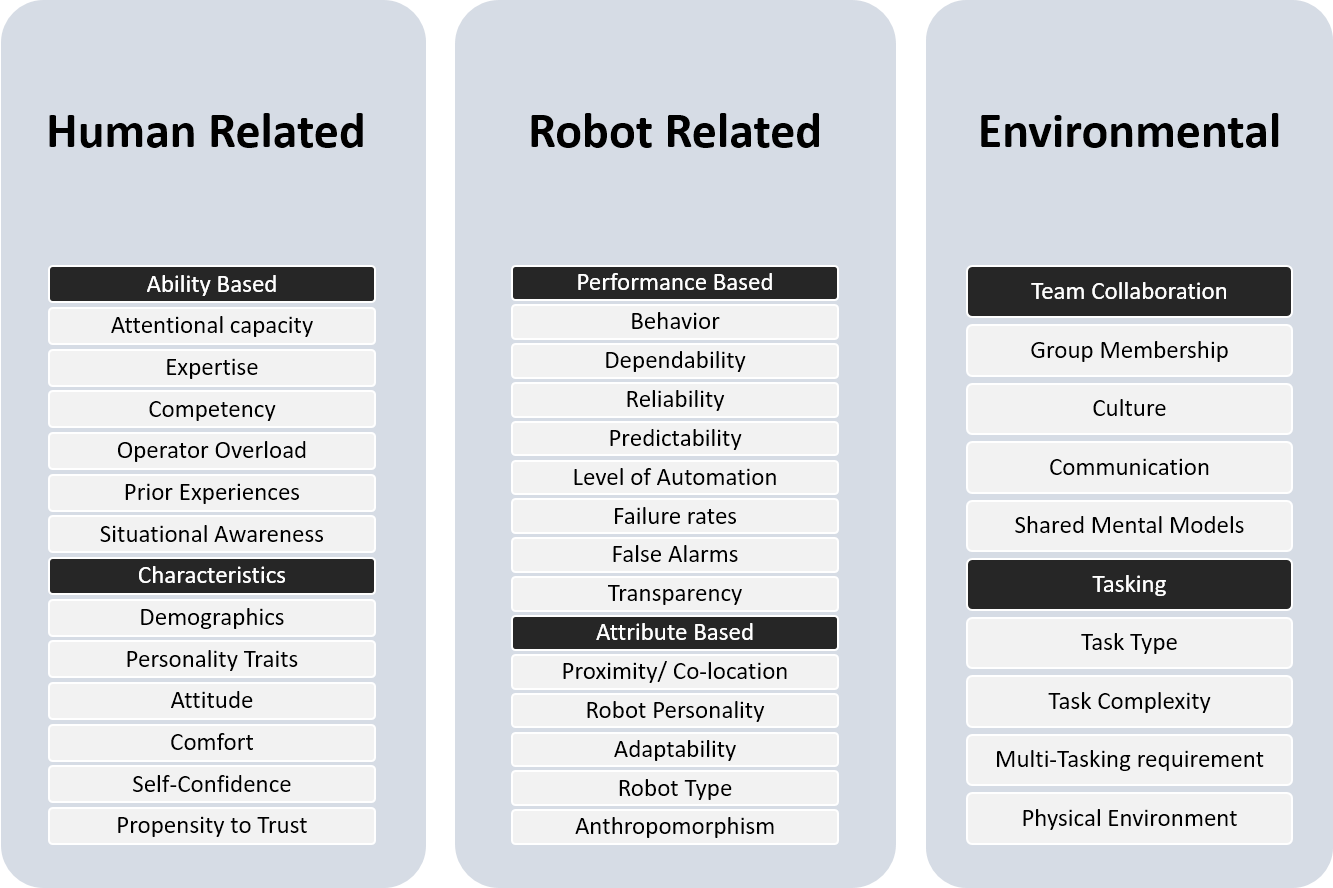
\includegraphics[width=\textwidth]{Figures/TrustFactors.png}
	\caption{Trust factors identified by Hancock \cite{hancock2011meta}}
\end{figure}

\newpage

Jacques Penders and his co-workers investigated HRI in `no-visibility' conditions \cite{penders2013enhancing}. No visibility condition in this context means that the human user might be visually impaired, or completely blind, therefore, they would have to completely trust the robot. This study also takes a look at the attributes in the design of robots that affect the ethical behavior of them. Additionally, this study analyzes the interaction of visually impaired person and their guide dog, and examines the variables that could be implemented in the design and behavior of robots to improve the human confidence in them. These variables include human dominance, cooperation overtime, and accountability.

In \cite{merritt2008not}, Stephanie Merritt at the University of Missouri examined the importance of taking differences in human behavior into consideration in the context of HRI. Ms. Merritt completed this empirical study by providing an experiment related to  X-ray screening. Subjects were asked to use a simulation software to detect dangerous items such as weapons, in different luggage. They given the options of scanning the x-ray image manually, and flagging it if they spot a suspicious item, or have a fictional autonomous system called  Automatic Weapons Detector(AWD) scan the image, and report any issues. This study concluded that the individual differences in subjects affects the value of trust in autonomous systems, even if the characteristics of the autonomous system is `constant'. Thus, this study suggests that future researchers in the field of HRI and trust should take human characteristics into consideration.

Raja Parasuraman and Christopher Miller investigated the concept of trust and etiquette in the domain of HRI \cite{parasuraman2004trust}. Given the fact that in many human-to-human social interaction scenarios, respect and etiquette highly influence the level of trust. Mr. Parasuraman and Mr. Miller argued that they also influence the perception of autonomous robots in humans. In this paper, etiquette is described as: ``the set of prescribed and proscribed behaviors
that permits meaning and intent to be ascribed to
actions.''. This study also provides an experiment related to the role of etiquette in HRI. In order to assess the influence of etiquette, test subjects used a flight simulator software called Multi-Attribute Task (MAT), and communicated with the autonomous system using different communication styles such as interrupting the user, being impatient, etc. The empirical evidence obtained by this experiment indicated that etiquette definitely influences the human trust, and reliability of autonomous robots.

A research conducted by Ms. Rosemarie Yagoda and her research partner, Mr. Douglas Gillan, provided a mechanism for measuring the value of trust in the context of HRI \cite{yagoda2012you}. This measurement is based on multiple factors, including team configuration, team processes, context, task, and system. This trust scale measuring mechanism is based on two studies in this research. In this first study, subject matter experts, and previous studies were used to construct a `content validity assessment'. The second study examines the trust scales obtained from the first study. The results of these two studies were combined to create the `HRI Trust Measuring Tool'.

In a 2014 paper, Yue Wang and partners investigated the human-robot trust in the context of underwater semi-autonomous robots \cite{wang2014human}. In order for the underwater robot to have a good performance, the person who is operating the robot needs to trust its autonomous capabilities. This study proposed a trust model that mainly deals with recording the robot's past performance, the human performance, and the fault rates of humans and robots. The semi-autonomous robot `YSI EcoMapper AUV' was investigated in this study specifically. Furthermore, MATLAB simulations indicate the effectiveness of this trust model.

In 1992, John Lee and Neville Moray explored the human-machine trust by studying the interactions of the users of a ``Semi-Automatic Pasteurization plant'' \cite{lee1992trust}. Based on the previous research, it had been known that the level of trust between humans and autonomous or semi-autonomous systems fluctuates depending on a variety of factors. For example, if was argued that some users didn't trust the new, semi-autonomous technology at all, and preferred to use the manual controls, instead of letting the autonomous system take care of the work. Some other users, interestingly, put ``too much'' trust in these systems, therefore, the risks of potential errors or faulty behavior caused by the system was possible. In the experiment provided by this paper, users were given the choices of operating a semi-automatic pasteurization plant for pasteurizing orange juice (simulation) using the manual mode, or the automatic-mode, or a combination of the mentioned two methods. This experiment indicated that the majority of users were able to adapt fairy quickly to this semi-automatic systems, however, when faulty behavior occurred, it was observed that the level of trust recovered more slowly. It was also concluded that the performance of the system significantly impacts the user's level of trust in the system.

\subsubsection{Human-Self Driving Cars (SDCs)}
Autonomous driving has been advancing exponentially in the recent years due to technological advancements in AI, mechanics and advanced sensor systems. Car manufacturers such as Google, Tesla, Mercedes-Benz, Ford, and many others have already created commercially available semi-autonomous cars, and fully autonomous prototypes, and they expect mass production of self driving cars (SDCs) in the early 2020s \cite{driverlessFutureForcast}. One major challenge in popularizing SDS in the US and the world would be the high level of distrust of average consumers in fully automated vehicles.

Daniel Howard at UC Berkeley (2013) \cite{howard2014public} explores the factors affecting the trust between humans and SDCs, and attempts to examine the attitude of average consumers towards SDCs in Berkeley, California. Mr. Howard's research indicates that most consumers have positive feelings toward the ease of use that comes with SDCs. In a fully autonomous vehicle, they wouldn't have to feel frustrated when driving in heavy traffic, or finding parking in a busy area due to the benefit of multitasking. One can imagine that at some time in the near future, commuters will be able to take naps, or watch movies while the SDC drives them to wherever they desire. Mr. Howard's also discovered that most individuals have concerns regarding the cost, liability, and the potential loss of control of SDCs. This study also indicated that factors such as level of income and gender affect the consumer's concerns. For example, subjects with higher levels of income were more concerned about liability as opposed to subjects with lower levels of income that were more concerned about the control of SDCs.

An experiment  conducted by William Payre and his team analyzed how alternating levels of trust would impact a driver's reaction time \cite{payre2016fully}.  The purpose of this experiment was to test the time between Manual Control Recovery (MCR) when emergency situations arose with Fully Automated Driving cars (FAD's).  Cars that are FAD's are certified and eligible to be used by drivers with a standard driver's license.  Nonetheless, the drivers are still accountable for their vehicle and regaining MCR in case of emergency, as well as being in the drivers seat with their seat belt buckled at all times.  Participants were asked to take a questionnaire prior to the simulation, as well as another one after the simulation.  The simulation was divided into three rounds that allowed researchers to test the reaction time between users being warned 30 seconds ahead of time to engage in MCR, and drivers upon emergency situations, in which they would have no warning ahead of time.  The first round allowed users to familiarize themselves with the controllers, the second had users starting the cars, as well as getting them up to 130 kmp until they were signaled to commence the FAD system and then engage in MCR, and the third gave users an emergency situation in which drivers had to engage in MCR as quickly as possible.  This study demonstrated that higher trust levels in the FAD's resulted in slower reaction times, which can create a hazardous environment for drivers who are complacent.  This experiment helped companies become more aware of the problems that over trust can cause, as well as simulate ideas for courses regarding gaining knowledge in MCR.

Michelle Carlson and her team, in a 2014 paper, provided a statistical analysis in the domain of autonomous vehicles and autonomous diagnostic systems \cite{carlson2014identifying}. Their goal was to identify the major factors that impact level of trust in self driving cars and autonomous medical systems. In this study an online survey was performed in which subjects were asked about various scenarios related to self driving cars. They were also asked about the use of IBM Watson in critical medical situations (e.g determining types of cancer). It was discovered that most test subjects were having concerns regarding the past performance of the car, reliability, errors, software/hardware failure, and the liability manufacturer of the car (e.g Google, or a lesser-known company). Similarly, it was discovered that the top factors that affect the trust in the use of IBM Watson in critical medical situations are the accuracy and past performance among many other factors. This indicates that regardless of the domain, most people tend to prioritize safety, accuracy, and failure rate when trusting an autonomous system.

In a similar study \cite{kyriakidis2015public}, Miltos Kyriakidis and his team created an international questionnaire related to the public opinion of automated driving. Questions included concerns, acceptance, and willingness to buy the car. Among the 5000 responders from 109 countries, most subjects agreed that fully automated self driving cars have the potential to be very popular among consumers by 2050. It was discovered that most subjects were concerned about safety, malicious activities/hacking, and legal issues related to autonomous driving. Mr. Kyriakidis also discovered that most of the subjects that were more educated, had more income, and were located in developed countries, were mostly uncomfortable about the self driving car transmitting data to external sources, and were concerned about the misuse of the transmitted data.

A 2015 study by Michael Wagner and Philip Koopman explored the possibilities of developing trust in Self Driving Cars using tools and techniques that are currently available \cite{wagner2015philosophy}. This study argues that fully autonomous Driving Cars aim to make our lives easier, and reduce the number of accidents. However, in many situations such as unpredictable hazards, and intense weather situations, the human driver's reactions are superior. This is one of the major factors that affects the human trust in Self Driving Cars. It is stated that testing is a critical aspect of determining if the car is trustworthy enough to be on the road, or has the potential to develop its trust over time. This paper also claims that these cars use Machine Learning and Image Processing to provide some functions, like detecting pedestrians. It was argued, however, that Self Driving Cars need a very high accuracy in their algorithms (close to 100\%), but Machine Learning algorithms are not capable of producing such accurate results. Mr. Wagner and Mr. Koopman bring to light a new software testing philosophy based on philosopher, Karl Popper's concept of `Falsification'. Falsification means: ``For any hypothesis to have credence, it must be inherently disprovable before it can become accepted as a scientific hypothesis or theory.''\cite{falsifiability}. Falsifiability helps testing because it causes testers to discover more flaws and vulnerabilities in Self Driving Cars. Thus, by improving, and reliability, the trust in them will increase over time.

Tove Helldin and colleagues at the University of Skövde in Sweden conducted a study related to the ability of SDCs in snow conditions \cite{helldin2013presenting}. In this study, 59 drivers were chosen to sit in an autonomous simulator cockpit. One group of drivers were given information about the risks and uncertainties of the SDCs when driving in heavy snow conditions, and the other group of drivers, were not given any information regarding the ability of the SDC. This experiment indicated that the group of drivers that were provided with the information about the risks and uncertainties did not trust the SDC, and preferred to override the system to manually drive the car. The other group, however, were not as prepared to override the autonomous system to drive the car manually, and had more trust in the system.


\subsubsection{Human-Autopilot Modes}
Scott Winter and colleagues \cite{winter2015indian} explored this low level of trust in the context of humans trusting autonomous aircraft. Subjects were asked if they preferred to be on a commercial plane with two pilots (a pilot and a copilot), a plane with a pilot in the cockpit and the copilot remotely working, or a plane with both pilots remotely controlling the aircraft. Mr. Winter and colleagues discovered that the subjects express a high degree of discomfort if they were on a fully autonomous commercial plane with both pilots just overseeing the movements and controlling the airplane remotely. They also discovered that subjects also expressed a low level of trust when only one pilot is in the cockpit and another one controlling the aircraft remotely. In this study, it was also concluded that the level of trust between humans and autonomous aircrafts is potentially related to the culture of humans. For example, it was discovered that test subjects from India feel more comfortable if they were on a fully autonomous aircraft, as opposed to subjects from the United States. Mr. Winter and colleagues found out that this difference could be due to the collectivist Indian culture, as apposed to the Individualist American culture.

Vadim Butakov and his colleague, Petros Ioannou, in \cite{butakov2015driving} suggest that the level of comfort and trust of users will increase if the design and dynamics of autopilot systems in cars are closer to what they are used to in regular cars. In this study, Mr. Butakov and Mr. Ioannou analyze and present a methodology that allows custom modification of autopilot modes such as  Adaptive Cruise Control (ACC) and automatic lane change systems based on individual preferences. They also support their proposed methodology by collecting data from an experimental vehicle.

At the The European Organization for the Safety of Air Navigation (\cite{kelly2003guidelines}), a study was conducted on the human trust in air trafic management systems (ATMs), and provides guidelines and strategies to improve this trust over time. This paper argues that currently, air traffic control operators use many automated and semi-automated computer tools, and it is expected that the use of automation in this context will rise in the near future. Thus, operators will have to trust highly autonomous (or fully autonomous) ATMs such as radar systems and communication tools. The procedure to improve the mentioned trust is broken down in multiple ``development phases'':
\begin{itemize}
	\item Developing ATMS using experienced air traffic controllers
	\item Providing high quality simulations
	\item Providing training for the controllers
	\item Transitioning period for the controllers
	\item Keeping the old technology in case failure
\end{itemize}

\subsubsection{Human-Agents(software agents)}
With the fast-paced advancements in the field of IT, software agents have become very important assets that help humans with the variety of tasks such as automating repetitive computing tasks, or assisting users with simple things, such as managing their emails. There are also agents capable of doing complex tasks by themselves, without the aid of users. Examples of such agents include automatic shopping assistants, customer help desks, and web robots \cite{IntelligentAgent}. As these software agents grow over time, and their level of complexity increases, the issue of trust in software agents becomes one of many challenges of the use of these agents in sensitive areas. In the movie Resident Evil (2002), there is a powerful software agent called `The Red Queen', who is in charge of a huge underground facility. Due to a bio-hazard outbreak, the Red Queen murders all the employees in the facility in order to contain the virus. Although Resident Evil is a fictional movie, it conveys an interesting concept regarding human-agent trust. In real life, Agents may become so complex that they will be able to take control of facilities or weapon systems. Thus, the level of trust in them becomes a primary concern.

In order to proceed, we need to define what an `agent' exactly is in this context, because it is a broad term. In one major study on software agents, Dr. Hyacinth Nwana defines Software agents as computer programs that have the capability to act on someone's behalf, and the ability to make various choices by themselves \cite{nwana1996software}. In their paper `Software Agents: An Overview', Dr. Nwana provides a detailed overview, and classification of software agents. He and his colleagues have identified three primary attributes that software agents should have: Autonomy, Learning, and cooperation. Autonomy in this case is described as ``The principle that agents can operate on their own without the need for human guidance''. `cooperation' refers to the concept of multiple agents communicating, and cooperating (I will explain this in detail in the later section dedicated to multi-agent systems). The last primary attribute, `learning'' is necessary because agents need to learn, and absorb external information in order to communicate, and respond to different situations.

Dr. Nwana demonstrates that Agents also have attributes that are considered to be secondary. Attributes such as versatility (Engaging in a variety of tasks), helpful behavior, truthfulness, and the level of human-trust in them (which is what we are interested in).

Dr. Nwana identifies seven types of agents in their research:
\begin{enumerate}
	\item Collaborative agents
	\item Interface agents
	\item Mobile agents
	\item Information/Internet agents
	\item Reactive agents
	\item Hybrid agents
	\item Smart Agents
\end{enumerate}

\begin{figure}
	\centering
		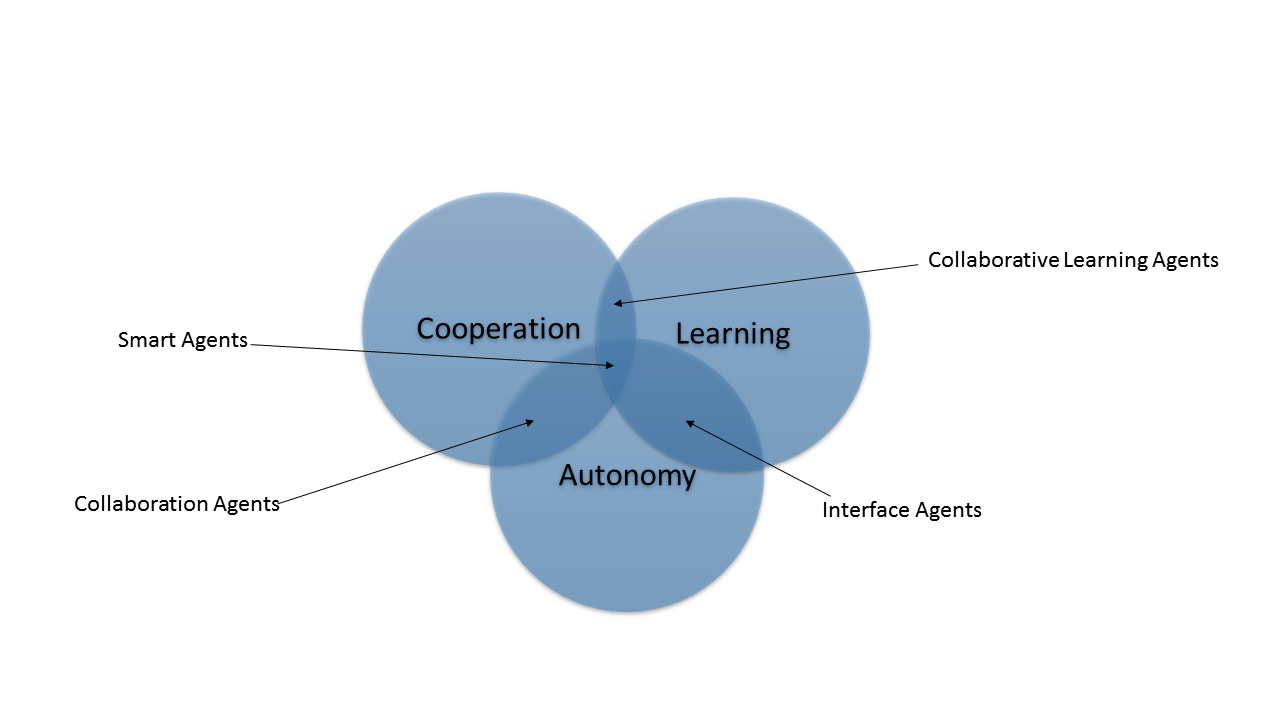
\includegraphics[width=\textwidth]{Figures/agents.png}
	\caption{Dr. Nwana's three primary attributes of agents (Dept. of IECS, Feng Chua University, R.O.C., 2003.)}
\end{figure}

In a study at MIT, Mr. Timothy Bickmore and his partner, Ms. Justine Cassell proposed an interesting model to build trust between users and computer agents \cite{bickmore2001relational}. Provided that in humans, trust is established and maintained by various social interactions such as small talk, Mr. Bickmore and Ms. Cassell argued that the same mechanism can also be used for computer agents to establish trust between users, and them. As an experiment, a computer agent called `REA' was used to communicate with users by performing small talk. REA was able to track the user's movements, and detect their emotional response. The experiment in this study yielded interesting results. It was discovered that users communicating with the REA system using small talk, who also happened to have extrovert personalities, had developed more trust than other users who had more introvert personality traits.

Mr. Bickmore's study indicates that the personality of users can potentially impact the level of trust between humans and agents. An older study conducted on the business school students in California State University yielded similar results. It was discovered that the level of self-esteem in human subjects plays a significant role in their performance and their interaction with a `human-like' computer: ``persons high in self-esteem generated more negative cognitive responses and made fewer errors when faced with human-like rather than machine-like feedback from a computer.'' \cite{resnik1985influence}

A study at University College London titled `Supporting Trust in Virtual Communities' proposes a reputation based trust model designed for improving trust in virtual communities. This trust model is based on `sociological characteristics of trust', such as past experiences and reputation, or `word of mouth'. This proposed model enables agents to take another agent's opinions and recommendations into consideration: ``Our
proposed model allows agents to decide which other
agents’ opinions they trust more and allows agents to
progressively tune their understanding of another agent’s
subjective recommendations.''  Mr. Abdul-Rahman and his colleague, Mr. Hailes argue that although this trust model is designed for increasing trust between humans and virtual societies, this trust model can also be implemented for artificial autonomous agents, and `artificial societies' \cite{abdul2000supporting}.


\subsubsection{Information Security}
At the The Norwegian University of Science and Technology, Mr. Audun Josang published a paper that aimed to focus on the concept of `trust' in the context of information security, and shed some light on the complex nature of Trust. He also examined various types of trust, and trust driven relationships that are relevant in the context of information security, and distributed systems. Mr. Josang provides an interesting definition of trust by defining it from a malicious point of view. He explains that essentially, trust occurs due to the tendency of humans to avoid malicious behaviors of agents (Other people or software). This concept of trust and detecting malicious behavior is critical in computer security due to potential hackers or agents attempting to penetrate a system. He also explores trust and malicious behavior from a philosophical point of view. \cite{josang1998modelling}


A 2006 study by Florina Almenarez et al. proposed a model for managing trust called `Pervasive Trust Management (PTM)' \cite{almenarez2006developing}. `Pervasive' devices are devices which are cumputing at all times. Apple Watches, smart-phones, PDAs etc. are examples of pervasive devices, which have microprocessors that compute things at all times in any network. The increased popularity of such devices produces the issue of trust between these devices communicating with each other, or providing a trusted, secure connection with any network. In this study, Ms. Almenarez, and her colleagues provide a statistical and mathematical trust model to tackle this problem.
\newpage
\section{Summary}

%\begin{table}[]
%\centering
%\caption{My caption}
%\label{my-label}
\begin{center}
\setlength\LTleft{0pt}
\setlength\LTright{0pt}
%\begin{longtable}{@{\extracolsep{\fill}}|c|c|l|c|c}
\begin{longtable}{|c|c|p{4cm}|p{2cm}|p{2cm}|}
\hline
\multicolumn{5}{|c|}{List of Studies}                                                                                               \\ \hline
Category                        & Study & \multicolumn{1}{c|}{Summary}    & \multicolumn{1}{c|}{Technology} & \multicolumn{1}{c|}{Focus} \\ \hline
\multirow{8}{*}{Human - Robots} 
	& \cite{stormont2008analyzing}    
	&  Confidence plays an important role as well as trust,\ and The unpredictability of the robot affects trust  
	& Computer simulation based on a firefighting scenario                        
	& Military, Hazardous environments
	\\ \cline{2-5} 
	& \cite{esfandiari2001agents}     
	& Mathematical definition for trust, where trust is a variable T. Trust acquisition is the process or mechanism that allows the calculation and update of 'T'
	& trust propagation model                      
	& Math-based trust propagation. Trust acquisition
	\\ \cline{2-5} 
	& \cite{hancock2011meta}
	& The performance of the robot has the biggest impact on trust in the context of HRI
	& N/A (meta-analysis)
	& HRI
	\\ \cline{2-5}
	&  \cite{penders2013enhancing}
	& In order to enhance trust in HRI, a number of design choices need to be made
	& visually impaired person and a guide dog
	& Improving trust in HRI
	\\ \cline{2-5} 
	& \cite{merritt2008not}
	& Different people have different levels of trust toward robot despite its constancy
	& X-ray screening simulation             
	& User perceptions of trust
	\\ \cline{2-5} 
	& \cite{parasuraman2004trust}
	& Etiquette affects human trust and the reliability of autonomous robots
	& Flight simulator
	& Impact of etiquette on trust
	\\ \cline{2-5} 
	& \cite{yagoda2012you}
	& Created the HRI `Trust Measuring Tool'
	& Subject Matter Experts (SMEs)                
	& Trust measurement
	\\ \cline{2-5} 
	& \cite{wang2014human}
	& If the human trusts the robot, its performance increases
	& YSI EcoMapper autonomous underwater robot         
	& Semi-autonomous mutual trust
	\\ \hline
\multirow{5}{*}{Human SDC}      
	& \cite{howard2014public}  
	& Most consumers like SDC's. Different people have different trust issues                     
	& Survey based on a 10 minute video                        
	& Perception of user's trust in SDCs
	\\ \cline{2-5} 
	& \cite{carlson2014identifying}
	& Most people tend to prioritize safety, accuracy, and failure rates when trusting an autonomous system                       
	& Surveys using  Survey Monkey and Amazon’s Mechanical Turk                  
	& Trust in Automated Cars and Medical Diagnosis Systems               
	\\ \cline{2-5} 
	& \cite{kyriakidis2015public}
	& The geographic positioning and education of consumers affects the premises of their trust 
	& Internet-based survey                    
	& User willingness to buy SDCs
	\\ \cline{2-5} 
	& \cite{wagner2015philosophy}    
	& Users testing; relying and improving will increase their trust in the robot 
	& N/A (survey of existing methods)         
	& Safety for SDC software based on 'falsificationism'
	\\ \cline{2-5} 
	& \cite{helldin2013presenting}
	& If people know about the problems of a robot, they will probably override it to avoid them            
	& Driving Simulator by Volvo  
	& The uncertainty of SDCs in various scenarios            
	\\ \hline
	
	\multirow{2}{*}{Human-Autopilot Modes}    
	& \cite{winter2015indian}
	& Culture affects trust                        
	& Internet based survey               
	& Trust in autonomous and semi-autonomous auto pilot systems        
	\\ \cline{2-5} 
	& \cite{butakov2015driving}
	& People have an easier time trusting familiar things.                   
	& Data collection from an experimental SDC
	& Autopilot personalization
	\\ \hline
	
	\multirow{3}{*}{Human-Agents (Software) } 
	& \cite{nwana1996software}
	& Agents have secondary attributes that affect trust                    
	& N/A (Meta-Analysis)                
	& Overview of software agents and comparison            
	\\ \cline{2-5}
	& \cite{bickmore2001relational}
	& Small talk builds trust, especially with extroverted personalities. The personality of users can impact the level of trust between humans and robots.
	& Conversation agent REA
	& Building trust using social dialogue
	\\ \cline{2-5} 
	& \cite{abdul2000supporting}
	& Model designed to increase trust between agents and agents, and humans and agents                     
	& Reputation-based trust model (Word of mouth)            
	& Increasing trust in agents in virtual communities
	\\ \hline
	
	\multirow{2}{*}{Information Security } 
	& \cite{josang1998modelling}
	& Trust occurs due to the tendency of humans to avoid malicious behaviors of agents                   
	& N/A (Analysis)
	& Trust in IT and malicious agents
	\\ \cline{2-5} 
	& \cite{almenarez2006developing}
	& Mathematical trust model designed to tackle the issue of trust between agents, creating secure connections etc.    
	& Mathematical Trust Evolution Model                       
	& Trust between agents in Pervasive devices (such as smart-phones and PDAs)
	\\ \hline

%\end{tabular}
\end{longtable}
\end{center}

\section{Open Problems, Future Directions and Concluding remarks}
%\bibliographystyle{abbrv}
\bibliography{ShervinTrustSurvey}

\end{document}

